\section{Multigrid solver}
\label{sec:da_solver}

In this section a multigrid solver for the diffusion approximation is developed. Multigrid schemes are the most efficient iterative methods for solving diffusion-type equations. The core idea is to propagate the error on a coarse grid during each iteration and take that propagated error into account, when doing an iteration step on the original high resolution grid. Particularly useful is the fact that the multigrid method can be employed on any system of linear equations as long as so called restriction and interpolation operators are being provided. 

The automatic discretization machinery, which was developed as part of the $P_N$-solver in section~\ref{sec:pn_solver} takes arbitrary systems of potentially coupled, linear partial differencial equations as input. The diffusion equation, which has been derived in the previous section is such a linear scalar partial differential equation and therefore can be fed into the automated stencil code generation from section~\ref{sec:pn_solver} to produce valid stencil code (independent of mesh resolution).

The idea behind the multigrid method is to accelerate the convergence by using a coarse grid on which information propagates faster throughout the spatial domain. The coarse solution is then used for updating the original grid.
%\begin{figure}[h]
%\centering
%\missingfigure{multigrid mesh setup}
%\caption{TODO}
%\label{fig:da_solver_multigrid_mesh}
%\end{figure}

Quantities on the original fine mesh are denoted with the subscript $F$. Therefore the original system of equations is received:
\begin{align}
\nonumber
A_F\vec{u}_F = \vec{b}_F
\end{align}
The multigrid method is an iterative method. This is expressed with a superscript index $i$, which denotes the current multigrid iteration. The first step in the multigrid cycle is to partially converge the solution by applying a number of iterations of an iterative method, such as Conjugate-Gradient or Gauss-Seidel. The partially converged solution in the first multigrid cycle is denoted $\vec{u}_F^i$. Then the residual is computed on the fine mesh:
\begin{align}
\nonumber
\vec{r}_F^i = \vec{b}_F-A_F\vec{u}_F^i
\end{align}
The idea behind multigrid is to use the coarse grid to smooth out the error and use the result as a correction for the next iterations on the fine mesh. To facilitate this, the residual on the fine mesh is first transferred onto the coarse mesh. This is done by downsampling the fine mesh residual (often also called interpolation). This operation can be represented as a non-symmetric matrix $M$. Quantities on the coarse mesh are denoted with the subscript $C$:
\begin{align}
\nonumber
\vec{r}_C^i = M_{F\rightarrow C} \vec{r}_F^i
\end{align}
With bringing the residual onto the coarse mesh, the next step is to solve the correction equation to full convergence. The correction equation is derived by looking at the system on the coarse mesh, using the partially converged solution $\vec{u}_C^i$:
\begin{align}
\nonumber
A_C\vec{u}_C^i = \vec{b}_C
\end{align}
Rearranging this equation allows us to use the downsampled residual as the right hand side vector:
\begin{align}
\nonumber
\vec{b}_C - A_C\vec{u}_C^i = \vec{r}_C^i
\end{align}
When substituting $\vec{b}_C$ with $A_C\vec{u}_C=\vec{b}_C$ (using the fully converged yet unknown solution on the coarse grid $\vec{u}_C$) following is shown:
\begin{align}
A_C\vec{u}_C - A_C\vec{u}_C^i &= \vec{r}_C^i
\nonumber
\\
A_C\left(\vec{u}_C-\vec{u}_C^i\right) &= \vec{r}_C^i
\nonumber
\\
A_C\vec{e}_C^i &= \vec{r}_C^i
\label{eq:da_correction_equation}
\end{align}
The quantity $\vec{e}_C^i$ is the unknown error between the final solution $\vec{u}_C$ and its partially converged approximation $\vec{u}_C^i$. Equation~\ref{eq:da_correction_equation} is called the correction equation and is solved to full convergence. The computed error is upsampled onto the finer grid, using the upsampling operator $M_{C\rightarrow F}$:
\begin{align}
\vec{e}_F^i = M_{C\rightarrow F}\vec{e}_C^i
\nonumber
\end{align}
Using the upsampled error a correction step to the solution on the fine grid can be applied:
\begin{align}
\vec{e}_F^i &= \vec{u}_F - \vec{u}_F^i
\nonumber
\\
\vec{u}_F^{i+1} &= \vec{u}_F = \vec{e}_F^i + \vec{u}_F^i
\nonumber
\end{align}
This process is then repeated by starting a new multigrid iteration with the corrected approximation $\vec{u}_F^{i+1}$. In summary a single multigrid iteration consists of the following steps:
\begin{enumerate}
\item Solve the original system on the fine grid, using a small number of iteration steps to bring the solution $\vec{u}_F^i$ to partial convergence.
\item Compute the residual $\vec{r}_F^i=\vec{b}_F - A_F\vec{u}_F^i$ on the fine grid and transfer it onto the coarse grid $\vec{r}_C^i = M_{F\rightarrow C}\vec{r}_F^i$.
\item Solve the correction equation $A_C\vec{e}_C^i = \vec{r}_C^i$ for $\vec{e}_C^0$ to full convergence on the coarse grid.
\item Transfer the result to the fine grid $\vec{e}_F^i = M_{C\rightarrow F}\vec{e}_C^i$.
\item Use $\vec{e}_F^i$ to apply the correction $\vec{u}_F^{i+1} =  \vec{e}_F^i + \vec{u}_F^i$.
\end{enumerate}
This is a two-level multigrid step, which could be extended to more levels by applying the same idea recursively to the coarse mesh solve. This is often done, so that the linear system of the coarsest level is so small that a direct method for solving it can be applied very efficiently. This results in the characteristic V-cycle shown in figure~\ref{fig:da_solver_multigrid_vcycles}.
\begin{figure}[h]
\centering
%\missingfigure{multigrid v-cycle}
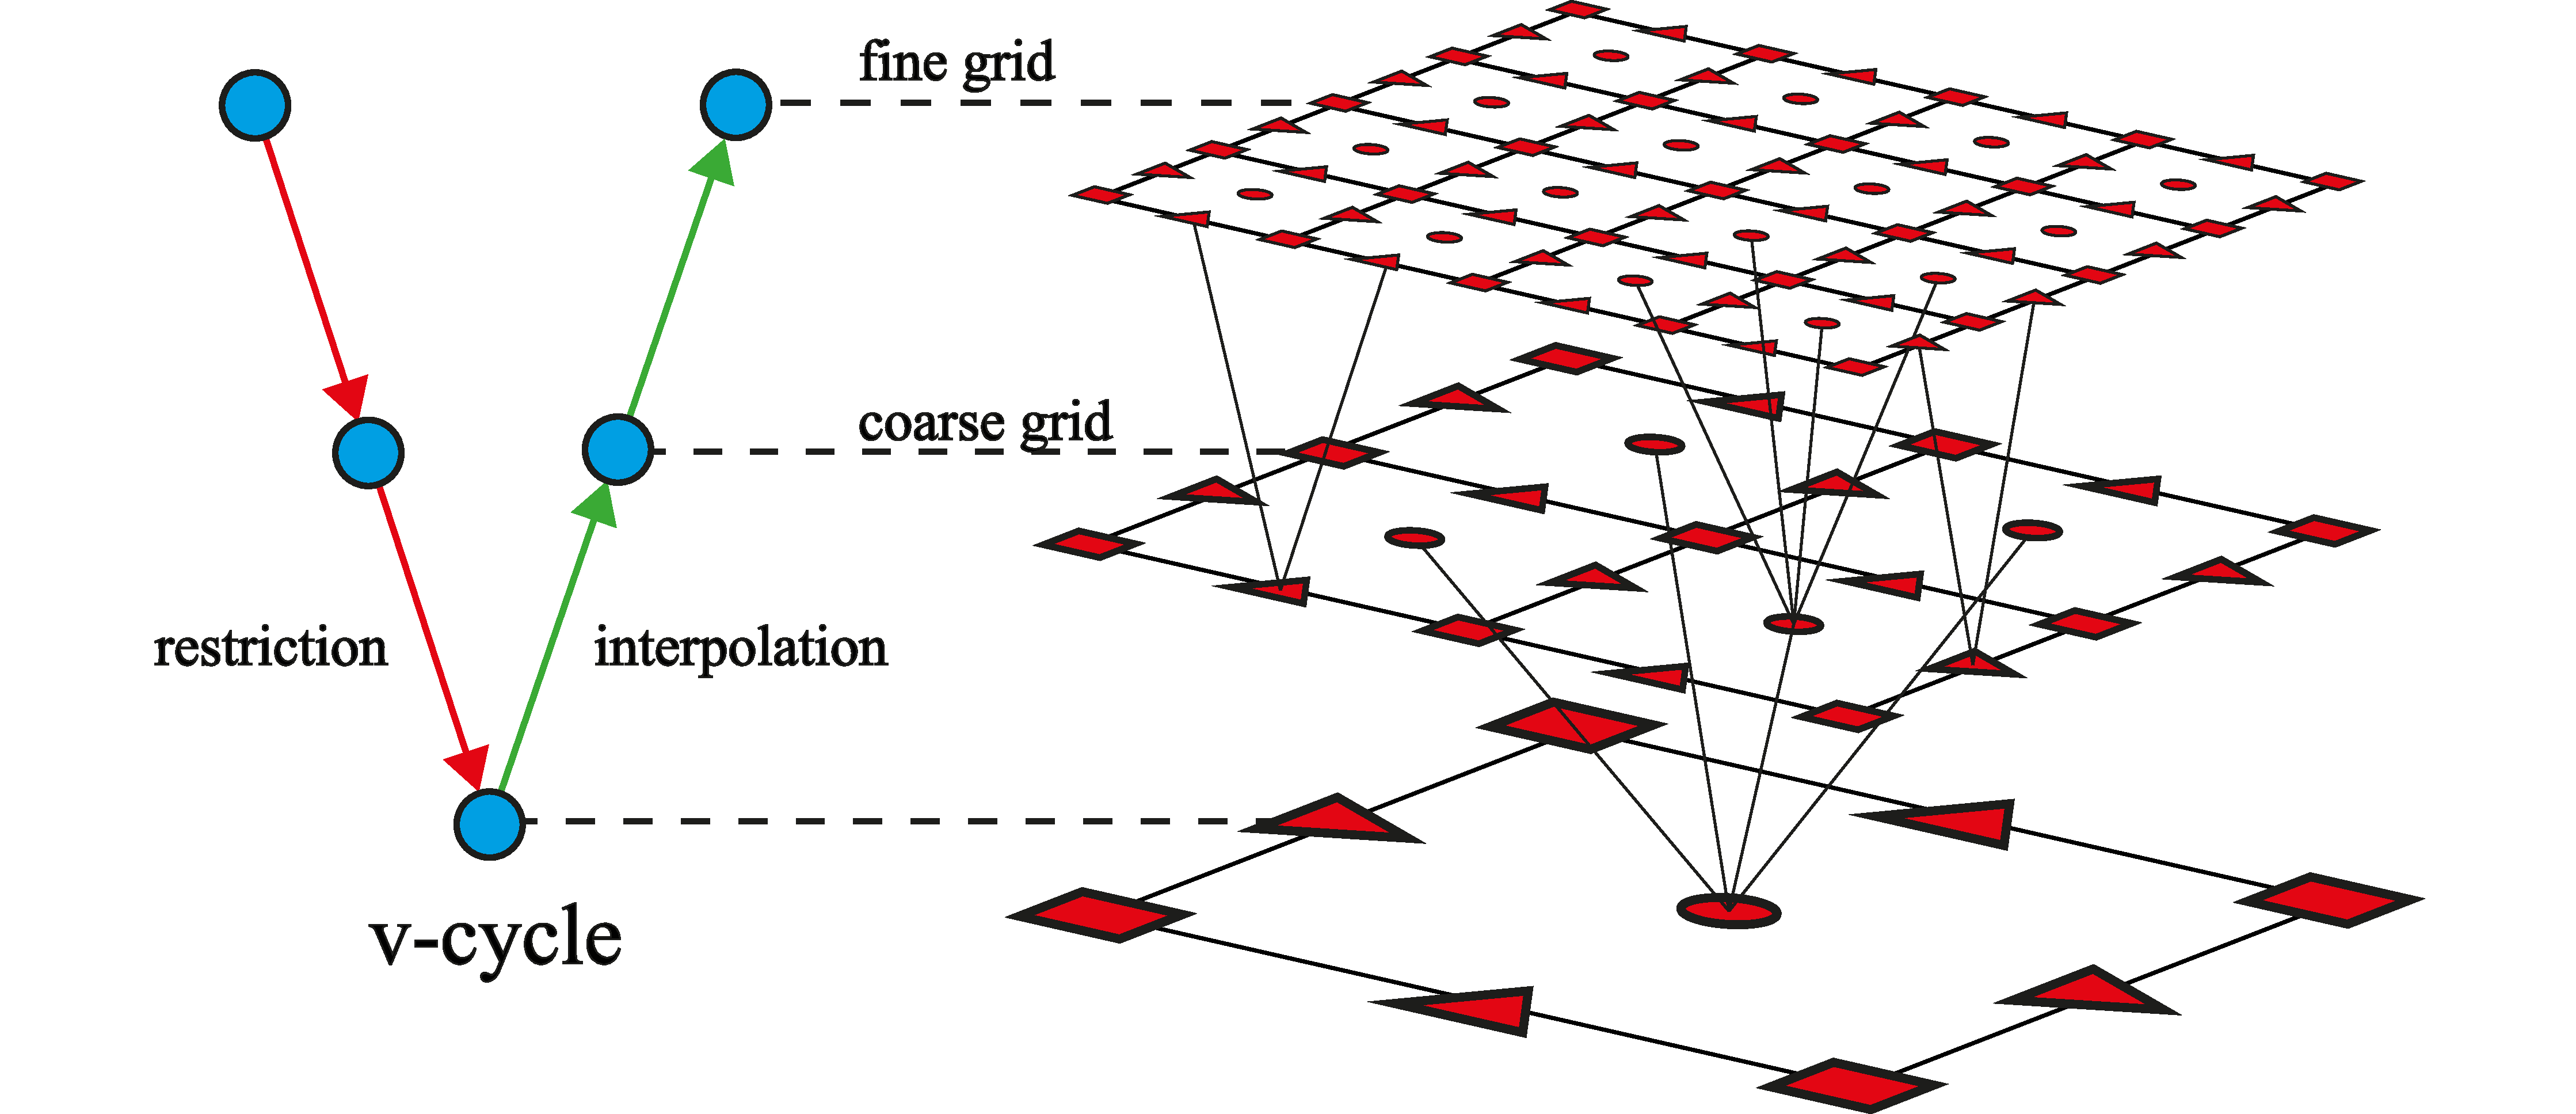
\includegraphics[width=0.85\textwidth]{05_diffusion_approximation/figures/fig_vcycle.pdf}
\caption{The staggered coarse grids for the multigrid v-cycle are computed from interpolating coefficients at their coarse grid locations.}
\label{fig:da_solver_multigrid_vcycles}
\end{figure}

Building the upsampling and downsampling matrices $M_{C\rightarrow F}$ and $M_{F\rightarrow C}$ is very similar to the problem of interpolating discretized variables at specific staggered grid locations for the automatic discretization in section~\ref{sec:pn_stencil_gen} (figure~\ref{fig:pn_discretization_interpolation}). In fact, the \emph{PNSystemBuilder} class presented in section~\ref{sec:pn_framework} has been extended to facilitate the automatic generation of the upsampling and downsampling operator matrices from a given discretization and a given vector of coefficients with their respective staggered grid locations. For the interpolation weights to not vary per voxel, the fine grid has to be exactly of double resolution. Further the number of multigrid levels defines the number of subdivisions required, and imposes additional constraints on the resolution. To support the maximum number of multigrid levels possible, the resolution has to be the power of two.
%\begin{figure}[h]
%\centering
%\missingfigure{interpolation matrix M, matrix layout, interpolation, throwing away coefficients}
%%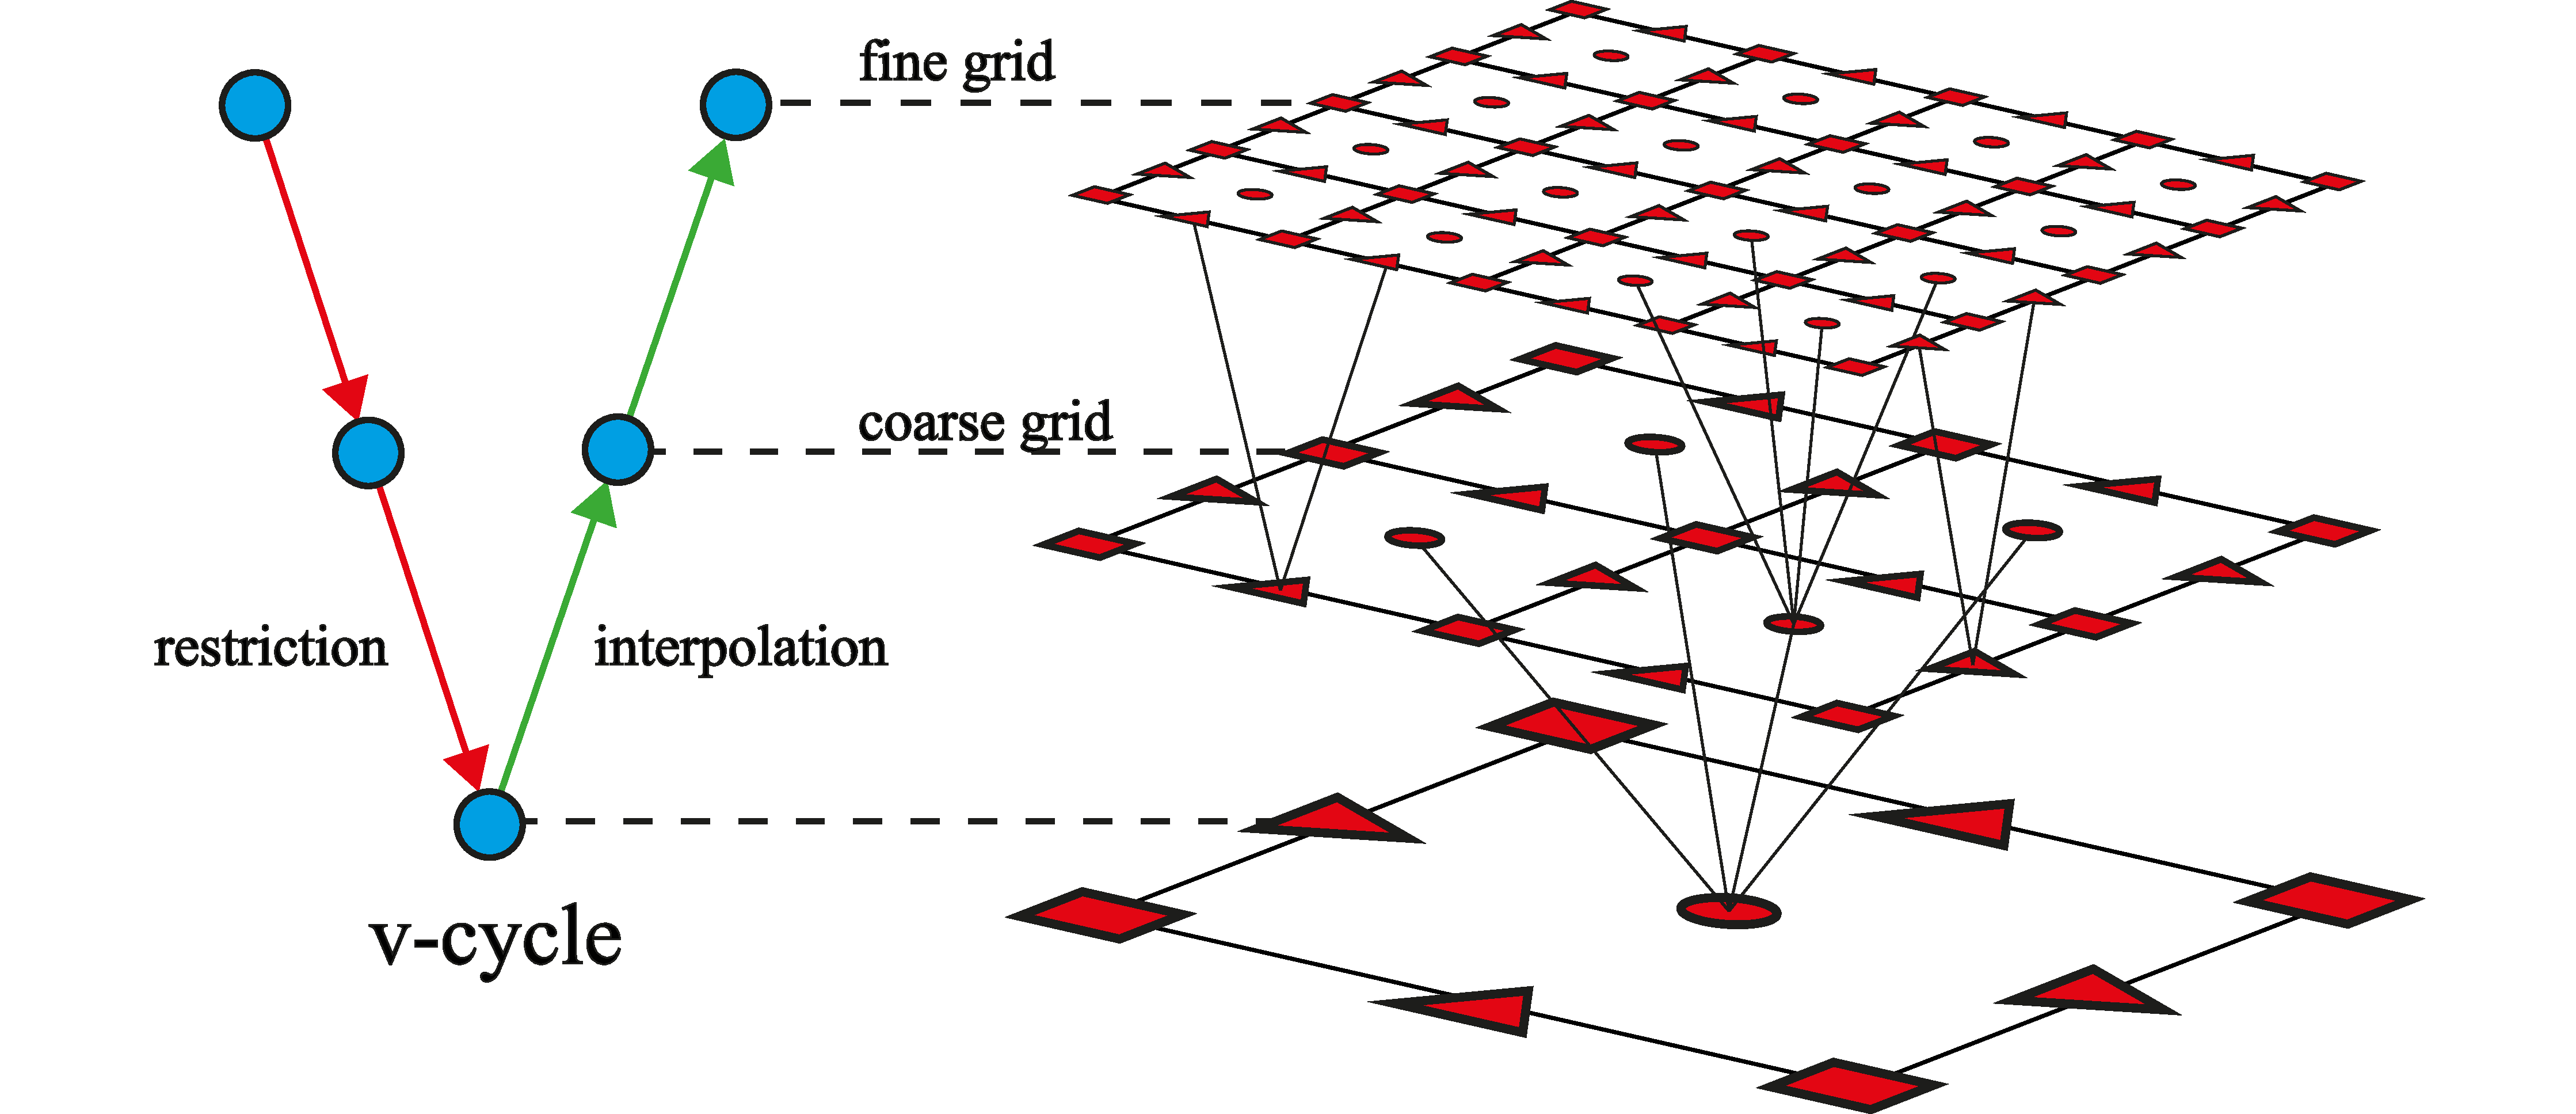
\includegraphics[width=0.6\textwidth]{05_diffusion_approximation/figures/fig_vcycle.pdf}
%\caption{TODO}
%\label{fig:da_solver_multigrid_M}
%\end{figure}

